% Options for packages loaded elsewhere
\PassOptionsToPackage{unicode}{hyperref}
\PassOptionsToPackage{hyphens}{url}
%
\documentclass[
]{article}
\usepackage{lmodern}
\usepackage{amssymb,amsmath}
\usepackage{ifxetex,ifluatex}
\ifnum 0\ifxetex 1\fi\ifluatex 1\fi=0 % if pdftex
  \usepackage[T1]{fontenc}
  \usepackage[utf8]{inputenc}
  \usepackage{textcomp} % provide euro and other symbols
\else % if luatex or xetex
  \usepackage{unicode-math}
  \defaultfontfeatures{Scale=MatchLowercase}
  \defaultfontfeatures[\rmfamily]{Ligatures=TeX,Scale=1}
\fi
% Use upquote if available, for straight quotes in verbatim environments
\IfFileExists{upquote.sty}{\usepackage{upquote}}{}
\IfFileExists{microtype.sty}{% use microtype if available
  \usepackage[]{microtype}
  \UseMicrotypeSet[protrusion]{basicmath} % disable protrusion for tt fonts
}{}
\makeatletter
\@ifundefined{KOMAClassName}{% if non-KOMA class
  \IfFileExists{parskip.sty}{%
    \usepackage{parskip}
  }{% else
    \setlength{\parindent}{0pt}
    \setlength{\parskip}{6pt plus 2pt minus 1pt}}
}{% if KOMA class
  \KOMAoptions{parskip=half}}
\makeatother
\usepackage{xcolor}
\IfFileExists{xurl.sty}{\usepackage{xurl}}{} % add URL line breaks if available
\IfFileExists{bookmark.sty}{\usepackage{bookmark}}{\usepackage{hyperref}}
\hypersetup{
  pdftitle={Homework 2},
  pdfauthor={Jake Underland},
  hidelinks,
  pdfcreator={LaTeX via pandoc}}
\urlstyle{same} % disable monospaced font for URLs
\usepackage[margin=1in]{geometry}
\usepackage{color}
\usepackage{fancyvrb}
\newcommand{\VerbBar}{|}
\newcommand{\VERB}{\Verb[commandchars=\\\{\}]}
\DefineVerbatimEnvironment{Highlighting}{Verbatim}{commandchars=\\\{\}}
% Add ',fontsize=\small' for more characters per line
\usepackage{framed}
\definecolor{shadecolor}{RGB}{248,248,248}
\newenvironment{Shaded}{\begin{snugshade}}{\end{snugshade}}
\newcommand{\AlertTok}[1]{\textcolor[rgb]{0.94,0.16,0.16}{#1}}
\newcommand{\AnnotationTok}[1]{\textcolor[rgb]{0.56,0.35,0.01}{\textbf{\textit{#1}}}}
\newcommand{\AttributeTok}[1]{\textcolor[rgb]{0.77,0.63,0.00}{#1}}
\newcommand{\BaseNTok}[1]{\textcolor[rgb]{0.00,0.00,0.81}{#1}}
\newcommand{\BuiltInTok}[1]{#1}
\newcommand{\CharTok}[1]{\textcolor[rgb]{0.31,0.60,0.02}{#1}}
\newcommand{\CommentTok}[1]{\textcolor[rgb]{0.56,0.35,0.01}{\textit{#1}}}
\newcommand{\CommentVarTok}[1]{\textcolor[rgb]{0.56,0.35,0.01}{\textbf{\textit{#1}}}}
\newcommand{\ConstantTok}[1]{\textcolor[rgb]{0.00,0.00,0.00}{#1}}
\newcommand{\ControlFlowTok}[1]{\textcolor[rgb]{0.13,0.29,0.53}{\textbf{#1}}}
\newcommand{\DataTypeTok}[1]{\textcolor[rgb]{0.13,0.29,0.53}{#1}}
\newcommand{\DecValTok}[1]{\textcolor[rgb]{0.00,0.00,0.81}{#1}}
\newcommand{\DocumentationTok}[1]{\textcolor[rgb]{0.56,0.35,0.01}{\textbf{\textit{#1}}}}
\newcommand{\ErrorTok}[1]{\textcolor[rgb]{0.64,0.00,0.00}{\textbf{#1}}}
\newcommand{\ExtensionTok}[1]{#1}
\newcommand{\FloatTok}[1]{\textcolor[rgb]{0.00,0.00,0.81}{#1}}
\newcommand{\FunctionTok}[1]{\textcolor[rgb]{0.00,0.00,0.00}{#1}}
\newcommand{\ImportTok}[1]{#1}
\newcommand{\InformationTok}[1]{\textcolor[rgb]{0.56,0.35,0.01}{\textbf{\textit{#1}}}}
\newcommand{\KeywordTok}[1]{\textcolor[rgb]{0.13,0.29,0.53}{\textbf{#1}}}
\newcommand{\NormalTok}[1]{#1}
\newcommand{\OperatorTok}[1]{\textcolor[rgb]{0.81,0.36,0.00}{\textbf{#1}}}
\newcommand{\OtherTok}[1]{\textcolor[rgb]{0.56,0.35,0.01}{#1}}
\newcommand{\PreprocessorTok}[1]{\textcolor[rgb]{0.56,0.35,0.01}{\textit{#1}}}
\newcommand{\RegionMarkerTok}[1]{#1}
\newcommand{\SpecialCharTok}[1]{\textcolor[rgb]{0.00,0.00,0.00}{#1}}
\newcommand{\SpecialStringTok}[1]{\textcolor[rgb]{0.31,0.60,0.02}{#1}}
\newcommand{\StringTok}[1]{\textcolor[rgb]{0.31,0.60,0.02}{#1}}
\newcommand{\VariableTok}[1]{\textcolor[rgb]{0.00,0.00,0.00}{#1}}
\newcommand{\VerbatimStringTok}[1]{\textcolor[rgb]{0.31,0.60,0.02}{#1}}
\newcommand{\WarningTok}[1]{\textcolor[rgb]{0.56,0.35,0.01}{\textbf{\textit{#1}}}}
\usepackage{graphicx,grffile}
\makeatletter
\def\maxwidth{\ifdim\Gin@nat@width>\linewidth\linewidth\else\Gin@nat@width\fi}
\def\maxheight{\ifdim\Gin@nat@height>\textheight\textheight\else\Gin@nat@height\fi}
\makeatother
% Scale images if necessary, so that they will not overflow the page
% margins by default, and it is still possible to overwrite the defaults
% using explicit options in \includegraphics[width, height, ...]{}
\setkeys{Gin}{width=\maxwidth,height=\maxheight,keepaspectratio}
% Set default figure placement to htbp
\makeatletter
\def\fps@figure{htbp}
\makeatother
\setlength{\emergencystretch}{3em} % prevent overfull lines
\providecommand{\tightlist}{%
  \setlength{\itemsep}{0pt}\setlength{\parskip}{0pt}}
\setcounter{secnumdepth}{-\maxdimen} % remove section numbering
\usepackage{amsmath}
\usepackage{dcolumn}
\usepackage{rotating}
\usepackage{amsmath}
\usepackage{dcolumn}
\usepackage{rotating}

\title{Homework 2}
\usepackage{etoolbox}
\makeatletter
\providecommand{\subtitle}[1]{% add subtitle to \maketitle
  \apptocmd{\@title}{\par {\large #1 \par}}{}{}
}
\makeatother
\subtitle{ECON 24450 Spring, 2021}
\author{Jake Underland}
\date{2021-04-27}

\begin{document}
\maketitle

{
\setcounter{tocdepth}{2}
\tableofcontents
}
\newcommand{\argmax}{\mathop{\mathrm{argmax}}}

\hypertarget{labor-supply-theory.}{%
\section{1. Labor Supply Theory.}\label{labor-supply-theory.}}

Using the lecture notes as a guide, show that 1) an increase in the wage
has an ambiguous effect on labor supply and 2) a traditional welfare
program unambiguously reduces labor supply.

\textit{Solution.}

\begin{enumerate}  
\item[1)]  

The uncompensated utility maximization problem: 
\[\begin{aligned}
\max_{x, l} u(x, l) \; \textit{ s.t. } \;px \leq y + w(T-l)
\end{aligned}\]

where $x$ is amount of goods consumed, $l$ is time spent on leisure, $T$ is total time, and $y$ is non-labor income.  
Solving the above,
\[\begin{aligned}
\max_{x, l} \mathcal{L} &= u(x, l) + \lambda [y + w(T-l) -px] \\
&[x]:\;u_x(x^*,l^*) - \lambda p = 0 \\
&[l]:\;u_l(x^*,l^*) - \lambda w = 0 \\
&[y]:\;y + w(T-l^*) -px^* = 0
\end{aligned}\]

In the optimal state, define 
\[\begin{aligned}
x^* &\equiv x^u(p,w,y)\\
l^* &\equiv l^u(p,w,y)\\
\lambda^* &\equiv \lambda(p,w,y)\\
h^u &\equiv T - l^* \dots \textit{(The uncompensated labor demand/supply)}\\
\epsilon_{h^u, w} &\equiv \frac{\partial h^u / h^u}{\partial w / w} = 
\frac{\partial h^u}{\partial w} \cdot \frac{w}{h^u} \textit{(The uncompensated labor demand/supply elasticity)}
\end{aligned}\]  
Now, we look at the dual expenditure minimization problem. 
\[\begin{aligned}
\min_{x, l} px + wl \; \textit{ s.t. } \;u(x, l) \geq \bar{u}
\end{aligned}\]
\[\begin{aligned}
\min_{x, l}\mathcal{L} &= px + wl  + \lambda [\bar{u}-u(x, l) ]\\
&[x]:\; p - \lambda u_x(x^*,l^*) = 0 \\
&[l]:\; w - \lambda u_l(x^*,l^*) = 0 \\
&[y]:\; \bar{u} - u(x^*, l^*) = 0
\end{aligned}\]  
In the optimal state, define 
\[\begin{aligned} 
\bar{u} &\equiv u(x^*, l^*) \\
x^* &\equiv u_x(p,w,\bar{u})\\
l^* &\equiv u_l(p,w,\bar{u})\\
h^c(p,w,\bar{u}) &\equiv T - l^c(p,w,\bar{u}) \dots \textit{(The compensated labor demand/supply)}\\
\epsilon_{h^c, w} &\equiv \frac{\partial h^c / h^c}{\partial w / w} = 
\frac{\partial h^c}{\partial w} \cdot \frac{w}{h^c} \textit{(The uncompensated labor demand/supply elasticity)}
\end{aligned}\]  
Now, we define the expenditure function $E(\cdot)$ and discuss its properties:
\[\begin{aligned}
E(p, w , \bar{u}) &\equiv p \cdot x^c(p,w,\bar{u}) + w\cdot l^c(p, w, \bar{u}) \\
&= p \cdot x^c(p,w,\bar{u}) + w\cdot (T - h^c(p, w, \bar{u})) \\
&=  \underbrace{p \cdot x^c(p,w,\bar{u}) - w\cdot h^c(p, w, \bar{u})}_{E^*(p, w, \bar{u}) \textit{(minimum needed value of non-labor income)}} + wT  \\
\end{aligned}\]
Now, differentiate $E^*(\cdot)$ w.r.t $w$ to yield 
\[\frac{\partial E^*}{\partial w} = \frac{\partial E(p, w, \bar{u})}{\partial w} - T\]
By the envelope theorem, 
\[= l^c(p, w, \bar{u}) - T = T - h^c - T = -h^c]\]
We can also derive concavity:
\[\begin{aligned}
\frac{\partial ^2}{\partial w^2} E^* &= \frac{\partial}{\partial w} - h ^c < 0 \\
&\implies \frac{\partial}{\partial w} h ^c > 0
\end{aligned}\]
The Slutsky Decomposition follows as: 
\[h^c(p, w, \bar{u}) = h^u(p,w,y) \]
where $y = E^*(p, w, \bar{u})$.  
Totally differentiate both sides of this equation w.r.t $w$ to get: 
\begin{align*}
\frac{\partial}{\partial w}h^c(p, w, \bar{u}) &= \frac{\partial}{\partial w}h^u(p,w,y) + \frac{\partial}{\partial y} h^u(p,w,y) \cdot \frac{\partial y}{\partial w} \\
&= \frac{\partial}{\partial w}h^u(p,w,E^*) + \frac{\partial}{\partial y} h^u(p,w,E^*) \cdot \frac{\partial E^*}{\partial w} \\
\implies  \frac{\partial h^c}{\partial w} &= \frac{\partial h^u}{\partial w} + \frac{\partial h^u}{\partial y} \cdot \underline{(-h^c)}_{\text{From Envelope theorem}}  \\
\implies  \frac{\partial h^u}{\partial w} &= \frac{\partial h^c}{\partial w} + \frac{\partial h^u}{\partial y} \cdot h^c \tag{$\star$}
\end{align*}
Where 
\[\begin{aligned}
&\frac{\partial h^u}{\partial y} = \frac{\partial (T - l^u(p,w,y))}{\partial y} = -\frac{\partial l^u}{\partial y} < 0 \dots \text{(Income Effect)} \\
&\frac{\partial h^c}{\partial w} > 0 \dots\text{(Substitution Effect)} \\
&h^c > 0
\end{aligned}\]
Thus, the substitution and income effect each work in the opposite direction in the final equation we have derived, rendering the effect of an increase in wage on labor supply ambiguous.  

\item[2)]  

Formulating the welfare program model:  
\[\begin{aligned}
G &= \text{max benefit}  \\
S &= G - t(wh) \dots \text{actual budget where $t$ is tax rate (benefit reduction)} \\
dw &= -tw \\
dy &= G
\end{aligned}\]
Totally differentiate uncompensated labor demand w.r.t $w$:
\[\begin{aligned}
\frac{d h^u}{dw} &= \frac{\partial h ^u}{\partial w} + \frac{\partial h ^u}{\partial y}\cdot \frac{dy}{dw} \\
\implies dh^u &=\frac{\partial h ^u}{\partial w}\cdot dw + \frac{\partial h ^u}{\partial y}\cdot dy
\end{aligned}\]
Plugging in $(\star)$, 
\[\begin{aligned}
dh^u &= (\frac{\partial h^c}{\partial w} + \frac{\partial h^u}{\partial y} \cdot h^c)(-tw) + \frac{\partial h ^u}{\partial y}\cdot dy \\
&= -tw\frac{\partial h^c}{\partial w} + \frac{\partial h^u}{\partial y}(-twh^c + dG) \\
\implies \frac{dh^u}{h} &= (-t)\cdot\frac{w}{h}\frac{\partial h^c}{\partial w} + \frac{\partial h^u}{\partial y}\frac{y}{h}(\frac{G-twh}{y})
\end{aligned}\]
Where $h = h^u = h^c$. 
\[\begin{aligned}
\implies \frac{dh^u}{h} &= \epsilon_{h^c,w}(-t) + \epsilon_{h^u, y} \cdot \frac{S}{y}
\end{aligned}\]
Where $\epsilon_{h^c,w} > 0$, $-t < 0$, $\epsilon_{h^u, y} < 0$, $\frac{S}{y} > 0$. Thus, the substitution effect $\epsilon_{h^c,w}(-t)$ of welfare and income affect $\epsilon_{h^u, y} \cdot \frac{S}{y}$ of welfare are both negative, and unambiguously reduce labor supply.

\end{enumerate}

\hypertarget{section}{%
\section{2.}\label{section}}

\break

\hypertarget{section-1}{%
\section{3.}\label{section-1}}

\break

\hypertarget{section-2}{%
\section{4.}\label{section-2}}

\break

\hypertarget{data-exercise}{%
\section{5. Data exercise}\label{data-exercise}}

\textit{In a few weeks, we will discuss disability insurance in detail. This data exercise is based on the paper The Impact of Economic Conditions on Participation in Disability Programs: Evidence from the Coal Boom and Bust (Black, Daniel, and Sanders 2002), which you should read before starting this question.}

\begin{Shaded}
\begin{Highlighting}[]
\KeywordTok{library}\NormalTok{(tidyr)}
\KeywordTok{library}\NormalTok{(dplyr)}
\KeywordTok{library}\NormalTok{(data.table)}
\KeywordTok{library}\NormalTok{(Hmisc)}
\KeywordTok{library}\NormalTok{(ivpack)}
\KeywordTok{library}\NormalTok{(stargazer)}
\KeywordTok{library}\NormalTok{(ggplot2)}
\end{Highlighting}
\end{Shaded}

\hypertarget{a.}{%
\subsection{a.}\label{a.}}

\textit{What is the causal relationship of interest in this paper? Write down the structural equation. Note: this equation does not appear in the paper.}

The paper estimates the marginal returns to medical care by
investigating the relationship between costs of medical inputs and child
mortality rates.

\[\Delta y = \alpha_0 + x\alpha_1 + \alpha_{2}\Delta (medical\:inputs) + \epsilon\]

Where \(y\) is child mortality rates.

\hypertarget{b.}{%
\subsection{b.}\label{b.}}

\textit{What is the problem with estimating this equation in cross-sectional data? In what direction is the estimate likely to be biased?}

Cross-sectional studies estimate returns to additional, incremental
spending that occur in some areas but not others, and on average find
similar health outcomes across section. However, they fail to account
for the endogenous correlation of the health risk of a population and
medical expenditure for that population. Thus, given the similarity in
health outcomes across sections, this type of study finds trouble
identifying a significant correlation between medical spending and
improvement of health outcomes. This likely biases the estimates
downward, towards the conclusion that the effect of medical spending on
mortality is null.

\hypertarget{c.}{%
\subsection{c.~}\label{c.}}

\textit{Fuzzy RD is just a form of IV. What is the instrument in this context? Explain how the instrument allows you to get an unbiased estimate of the causal relationship of interest.}

The instrument is the VLBW indicator. Assuming continuity of other
relevant factors contributing to an infant's mortality, infants that are
just below the threshold of \(1500g\) receive higher medical inputs
(summarized in medical expenditure) than infants just above due to
medical customs and guidelines. Thus, this instrument allows us to
isolate medical spending and overall medical inputs from the individual
infant's risk level, and show the effect that medical spending has on
infant mortality while controlling for health.

\hypertarget{d.}{%
\subsection{d.~}\label{d.}}

\textit{Write down the “first stage” regression discontinuity equation and the “reduced form” regression discontinuity equation. (These do appear in the paper.) Explain each term of the equations and the coefficients of interest.}

\[Y_i = \alpha_0 + \alpha_1 VLBW_i + \alpha_2 VLBW_i \times (g_i - 1500) + \alpha _3 (1-VLBW_i) \times (g_i - 1500) + \alpha_t + \alpha_s + \delta X_i ' + \epsilon_i\]

The first stage is when \(Y_i\) denotes costs and the reduced form is
when \(Y_i\) denotes the infant one-year mortality rate. \(VLBW_i\) is a
dummy variable that indicates whether an infant is classified as
\(VLBW\) (\(<1500g\)), and its coefficient \(\alpha_1\) indicates the
degree to which being \(VLBW\) affects mortality. The second and third
terms are gram trend terms below and above the threshold, parameterized
so that their coefficients are equal when the trends are the same.
\(\alpha_t\) and \(\alpha_s\) are indicators for the year of birth \(t\)
and state of birth \(s\). \(X_i '\) are the controls used that deal with
other newborn characteristics not specified in the rest of the model,
and \(\epsilon_i\) is the error term.

\hypertarget{e.}{%
\subsection{e.}\label{e.}}

\textit{Name one or more key threats to the validity of the empirical strategy used by Almond et al. (2010). Be specific to their context. Describe what tests you would perform to assess these threats.}

One threat is that the summary measures utilized for medical inputs may
not be exhaustive, and that unobserved factors that reduce mortality may
also contribute to the discontinuity in mortality around the 1500 g
threshold. For example, since the 1500 g. cut-off is well known in the
medical community, infants born under 1500 g. may be paid especially
close attention by physicians and medical staff, and treated with more
care than those who clear the 1500 g. line. This is outlined in Angert
and Adam (2009). Many of these behavioral changes in the medical staff
may not be picked up by the summary measure (medical costs), and result
in a slight upward bias. This threat can be analyzed by obtaining
records of infants just below and above the 1500 g. threshold with
identical treatment/medical input records and analyze for a notable
difference in their mortality.\\
Moreover, using the summary statistic of medical cost may run the risk
of overlooking price changes corresponding with weight, but as the
authors suggest in the paper, this threat can be tested by analyzing for
discontinuity in pricing across the VLBW threshold, among other methods.

\hypertarget{f.}{%
\subsection{f.~}\label{f.}}

\textit{Download the data set from: http://data.nber.org/lbid/adkw.dta. Import the data set to your preferred statistical analysis program (e.g., Stata, R). By downloading the data set, you agree to the following NCHS data rules: 1) Use the data in this dataset for statistical reporting and analysis only. 2) Make no use of the identity of any person or establishment discovered inadvertently and advise the Director, NCHS, of any such discovery. 3) Not link this dataset with individually identifiable data from other NCHS or non- NCHS datasets.}

\hypertarget{i.}{%
\subsubsection{i.}\label{i.}}

\textit{i. Replicate Figure 2-A, which gives the main finding of the paper.}

\hypertarget{a.-1}{%
\paragraph{A.}\label{a.-1}}

\textit{Group births into 1-ounce (28.3495-gram) bins, radiating outward from the 1500 gram threshold.}

\begin{Shaded}
\begin{Highlighting}[]
\CommentTok{# loading in data}
\NormalTok{dat <-}\StringTok{ }\KeywordTok{read.csv}\NormalTok{(}\StringTok{"DataExercise_RD/adkw.csv"}\NormalTok{)}
\end{Highlighting}
\end{Shaded}

\begin{Shaded}
\begin{Highlighting}[]
\CommentTok{# creating bin categories }
\NormalTok{ub <-}\StringTok{ }\KeywordTok{max}\NormalTok{(dat}\OperatorTok{$}\NormalTok{dbirwt)}
\NormalTok{lb <-}\StringTok{ }\KeywordTok{min}\NormalTok{(dat}\OperatorTok{$}\NormalTok{dbirwt)}
\NormalTok{s1 <-}\StringTok{ }\KeywordTok{seq}\NormalTok{(}\DataTypeTok{from =} \DecValTok{1500}\NormalTok{, }\DataTypeTok{to =}\NormalTok{ ub, }\DataTypeTok{by =} \FloatTok{28.3495}\NormalTok{)}
\NormalTok{s2 <-}\StringTok{ }\KeywordTok{rev}\NormalTok{(}\KeywordTok{seq}\NormalTok{(}\DataTypeTok{from =} \DecValTok{1500}\NormalTok{, }\DataTypeTok{to =}\NormalTok{ lb, }\DataTypeTok{by =} \FloatTok{-28.3945}\NormalTok{))}
\NormalTok{s2 <-}\StringTok{ }\KeywordTok{head}\NormalTok{(s2, }\DecValTok{-1}\NormalTok{)}
\NormalTok{bins <-}\StringTok{ }\KeywordTok{c}\NormalTok{(s2, s1)}
\NormalTok{bins <-}\StringTok{ }\KeywordTok{c}\NormalTok{(}\OperatorTok{-}\OtherTok{Inf}\NormalTok{, bins, }\OtherTok{Inf}\NormalTok{)}
\NormalTok{bin_groups <-}\StringTok{ }\KeywordTok{seq}\NormalTok{(}\DecValTok{1}\OperatorTok{:}\NormalTok{(}\KeywordTok{length}\NormalTok{(bins) }\OperatorTok{-}\StringTok{ }\DecValTok{1}\NormalTok{))}
\NormalTok{bins; bin_groups}
\end{Highlighting}
\end{Shaded}

\begin{verbatim}
## [1]     -Inf 1443.211 1471.605 1500.000 1528.350 1556.699      Inf
\end{verbatim}

\begin{verbatim}
## [1] 1 2 3 4 5 6
\end{verbatim}

\begin{Shaded}
\begin{Highlighting}[]
\CommentTok{# cutting data into bins }
\NormalTok{dat}\OperatorTok{$}\NormalTok{bwt_bins <-}\StringTok{ }\KeywordTok{cut}\NormalTok{(dat}\OperatorTok{$}\NormalTok{dbirwt, }\DataTypeTok{breaks =}\NormalTok{ bins, }\DataTypeTok{labels =}\NormalTok{ bin_groups)}
\end{Highlighting}
\end{Shaded}

\hypertarget{b.-1}{%
\paragraph{B.}\label{b.-1}}

\textit{For each bin, plot the bin’s mean one year mortality against the bin’s median birthweight.}

\begin{Shaded}
\begin{Highlighting}[]
\NormalTok{gdat <-}\StringTok{ }\NormalTok{dat }\OperatorTok
\StringTok{  }\KeywordTok{group_by}\NormalTok{(bwt_bins) }\OperatorTok
\StringTok{  }\KeywordTok{mutate}\NormalTok{(}\DataTypeTok{bin_medianwt =} \KeywordTok{median}\NormalTok{(dbirwt, }\DataTypeTok{na.rm =} \OtherTok{TRUE}\NormalTok{)) }\OperatorTok\StringTok{  }\CommentTok{# median bwt}
\StringTok{  }\KeywordTok{mutate}\NormalTok{(}\DataTypeTok{bin_meandeath =} \KeywordTok{mean}\NormalTok{(death1year, }\DataTypeTok{na.rm =} \OtherTok{TRUE}\NormalTok{)) }\OperatorTok\StringTok{  }\CommentTok{# mean mortality }
\StringTok{  }\KeywordTok{mutate}\NormalTok{(}\DataTypeTok{bin_meanage =} \KeywordTok{mean}\NormalTok{(gestat, }\DataTypeTok{na.rm =} \OtherTok{TRUE}\NormalTok{)) }\CommentTok{# mean gestational age}
\end{Highlighting}
\end{Shaded}

\begin{Shaded}
\begin{Highlighting}[]
\KeywordTok{ggplot}\NormalTok{(gdat, }\KeywordTok{aes}\NormalTok{(}\DataTypeTok{x =}\NormalTok{ bin_medianwt, }\DataTypeTok{y =}\NormalTok{ bin_meandeath)) }\OperatorTok{+}
\StringTok{  }\KeywordTok{geom_point}\NormalTok{(}\DataTypeTok{pch =} \DecValTok{16}\NormalTok{) }\OperatorTok{+}
\StringTok{  }\KeywordTok{xlim}\NormalTok{(}\DecValTok{1400}\NormalTok{, }\DecValTok{1600}\NormalTok{) }\OperatorTok{+}\StringTok{ }
\StringTok{  }\KeywordTok{geom_vline}\NormalTok{(}\DataTypeTok{xintercept =} \DecValTok{1500}\NormalTok{) }\OperatorTok{+}
\StringTok{  }\KeywordTok{labs}\NormalTok{(}\DataTypeTok{x =} \StringTok{"Birth weight (g)"}\NormalTok{, }\DataTypeTok{y =} \StringTok{"Mean 1 Year Mortality"}\NormalTok{) }\OperatorTok{+}
\StringTok{  }\KeywordTok{ggtitle}\NormalTok{(}\StringTok{"One Year Mortality"}\NormalTok{)}
\end{Highlighting}
\end{Shaded}

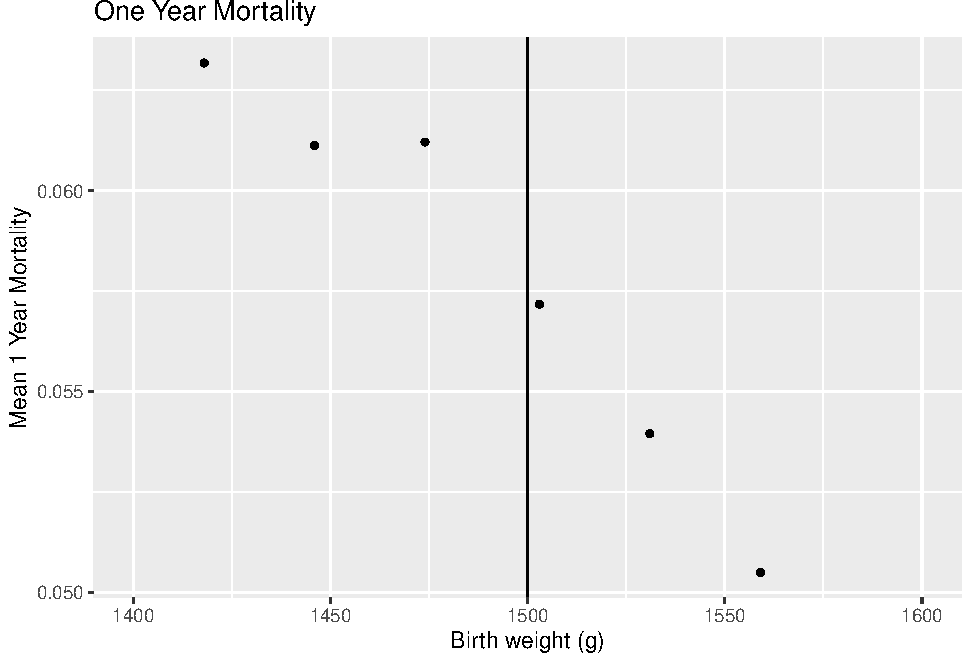
\includegraphics{Pset2_files/figure-latex/unnamed-chunk-5-1.pdf}

\hypertarget{c.-1}{%
\paragraph{C.}\label{c.-1}}

\textit{Interpret the graph you created, which is the main finding of the paper.}

Due to the limitations of our data, we are unable to observe the same
discontinuity that was observed in the paper. Mean mortality seems to be
continuous around the 1500g. line, and if there is a discontinuity it
seems to be between the bins with 1443.211-1471.605 g. and
1471.605-1500.000 g. Thus, replicating the analyses in the paper on this
data set may not be appropriate.

\hypertarget{ii.}{%
\subsubsection{ii.}\label{ii.}}

\textit{Test for differences in observable covariates across the 1500 gram threshold (replicate Figure
5-A from the paper).}

\hypertarget{a.-2}{%
\paragraph{A.}\label{a.-2}}

\textit{Adapt the method used in (i) to replicate Figure 5-A (the covariate of interest is gestational age).}

\begin{Shaded}
\begin{Highlighting}[]
\KeywordTok{ggplot}\NormalTok{(gdat, }\KeywordTok{aes}\NormalTok{(}\DataTypeTok{x =}\NormalTok{ bin_medianwt, }\DataTypeTok{y =}\NormalTok{ bin_meanage)) }\OperatorTok{+}
\StringTok{  }\KeywordTok{geom_point}\NormalTok{(}\DataTypeTok{pch =} \DecValTok{16}\NormalTok{) }\OperatorTok{+}
\StringTok{  }\KeywordTok{geom_vline}\NormalTok{(}\DataTypeTok{xintercept =} \DecValTok{1500}\NormalTok{) }\OperatorTok{+}
\StringTok{  }\KeywordTok{xlim}\NormalTok{(}\DecValTok{1400}\NormalTok{, }\DecValTok{1600}\NormalTok{) }\OperatorTok{+}\StringTok{ }
\StringTok{  }\KeywordTok{labs}\NormalTok{(}\DataTypeTok{x =} \StringTok{"Birth weight (g)"}\NormalTok{, }\DataTypeTok{y =} \StringTok{"Mean Gestational Age"}\NormalTok{) }\OperatorTok{+}
\StringTok{  }\KeywordTok{ggtitle}\NormalTok{(}\StringTok{"Gestational Age"}\NormalTok{)}
\end{Highlighting}
\end{Shaded}

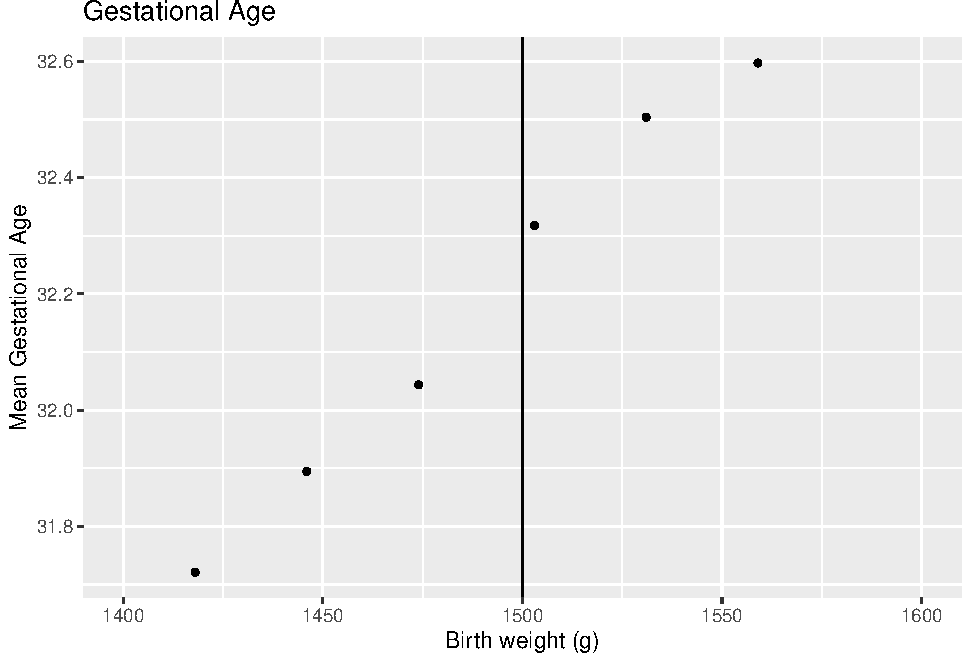
\includegraphics{Pset2_files/figure-latex/unnamed-chunk-6-1.pdf}

\hypertarget{b.-2}{%
\paragraph{B.}\label{b.-2}}

\textit{Which RD identifying assumption does this figure support? Explain.}\\
This graph shows continuity of other covariates that likely contribute
to child mortality around the 1500 g. line. Continuity in the covariates
allows us to assume that the only factor contributing to the
discontinuity observed in the original data is the binary indicator of
whether a child crosses the 1500 g. threshold or not, which acts as a
proxy for quantity of medical inputs received by the infant. Without
this assumption, there may be underlying factors contributing to the
discontinuity and our research design will not be able to isolate and
pick up the effects of medical inputs on child mortality.

\hypertarget{iii.}{%
\subsubsection{iii.}\label{iii.}}

\textit{Above, you wrote down the reduced form equation that appears in the paper.}

\break

\hypertarget{a.-3}{%
\paragraph{A.}\label{a.-3}}

\textit{Construct a dummy variable $VLBW_i$ that equals one if the infant is classified as very low birthweight (i.e., birthweight strictly less than 1500 grams), and 0 otherwise.}

\begin{Shaded}
\begin{Highlighting}[]
\CommentTok{# creating dummy }
\NormalTok{dat <-}\StringTok{ }\NormalTok{dat }\OperatorTok
\StringTok{  }\KeywordTok{mutate}\NormalTok{(}\DataTypeTok{VLBW =} \KeywordTok{ifelse}\NormalTok{(dbirwt }\OperatorTok{<}\StringTok{ }\DecValTok{1500}\NormalTok{, }\DecValTok{1}\NormalTok{, }\DecValTok{0}\NormalTok{),}
         \DataTypeTok{trend.down =}\NormalTok{ VLBW }\OperatorTok{*}\StringTok{ }\NormalTok{(dbirwt }\OperatorTok{-}\StringTok{ }\DecValTok{1500}\NormalTok{), }
         \DataTypeTok{trend.up =}\NormalTok{ (}\DecValTok{1} \OperatorTok{-}\StringTok{ }\NormalTok{VLBW) }\OperatorTok{*}\StringTok{ }\NormalTok{(dbirwt }\OperatorTok{-}\StringTok{ }\DecValTok{1500}\NormalTok{))}
\end{Highlighting}
\end{Shaded}

\hypertarget{b.-3}{%
\paragraph{B.}\label{b.-3}}

\textit{Ignore the terms $\alpha _t$, $\alpha_s$ and $\delta X_i$ in the reduced form equation. Estimate the reduced form equation by OLS. Obtain heteroskedastic-robust standard errors.}

\begin{Shaded}
\begin{Highlighting}[]
\CommentTok{# OLS estimate}
\NormalTok{reduced.ols <-}\StringTok{ }\KeywordTok{lm}\NormalTok{(death1year }\OperatorTok{~}\StringTok{ }\NormalTok{VLBW }\OperatorTok{+}\StringTok{ }\NormalTok{trend.down }\OperatorTok{+}\StringTok{ }\NormalTok{trend.up, }\DataTypeTok{data =}\NormalTok{ dat)}
\end{Highlighting}
\end{Shaded}

\begin{Shaded}
\begin{Highlighting}[]
\CommentTok{# Heteroskedastic robust standard errors }
\NormalTok{hkse <-}\StringTok{ }\ControlFlowTok{function}\NormalTok{(reg)\{}\KeywordTok{robust.se}\NormalTok{(reg)[,}\DecValTok{2}\NormalTok{]\}}
\NormalTok{ols_error <-}\StringTok{ }\KeywordTok{hkse}\NormalTok{(reduced.ols)}
\end{Highlighting}
\end{Shaded}

\begin{verbatim}
## [1] "Robust Standard Errors"
\end{verbatim}

\hypertarget{c.-2}{%
\paragraph{C.}\label{c.-2}}

\emph{Construct a table that contains the estimated coefficients
\(\hat{\alpha}_1, \hat{\alpha}_2, \hat{\alpha}_3\) from the reduced form
equation. Report standard errors in parentheses below each estimate. In
your table, indicate whether each estimated coefficient is significant
at a 1\%, 5\% or 10\% level.}

\begin{Shaded}
\begin{Highlighting}[]
\KeywordTok{stargazer}\NormalTok{(reduced.ols, }\DataTypeTok{type=}\StringTok{"latex"}\NormalTok{, }\DataTypeTok{title =} \StringTok{"OLS Results"}\NormalTok{, }
          \DataTypeTok{se =} \KeywordTok{list}\NormalTok{(ols_error), }\DataTypeTok{header =} \OtherTok{FALSE}\NormalTok{, }\DataTypeTok{no.space=}\OtherTok{TRUE}\NormalTok{)}
\end{Highlighting}
\end{Shaded}

\begin{table}[!htbp] \centering 
  \caption{OLS Results} 
  \label{} 
\begin{tabular}{@{\extracolsep{5pt}}lc} 
\\[-1.8ex]\hline 
\hline \\[-1.8ex] 
 & \multicolumn{1}{c}{\textit{Dependent variable:}} \\ 
\cline{2-2} 
\\[-1.8ex] & death1year \\ 
\hline \\[-1.8ex] 
 VLBW & $-$0.010$^{***}$ \\ 
  & (0.002) \\ 
  trend.down & $-$0.0001$^{***}$ \\ 
  & (0.00003) \\ 
  trend.up & $-$0.0002$^{***}$ \\ 
  & (0.00003) \\ 
  Constant & 0.063$^{***}$ \\ 
  & (0.001) \\ 
 \hline \\[-1.8ex] 
Observations & 202,071 \\ 
R$^{2}$ & 0.001 \\ 
Adjusted R$^{2}$ & 0.0005 \\ 
Residual Std. Error & 0.233 (df = 202067) \\ 
F Statistic & 33.752$^{***}$ (df = 3; 202067) \\ 
\hline 
\hline \\[-1.8ex] 
\textit{Note:}  & \multicolumn{1}{r}{$^{*}$p$<$0.1; $^{**}$p$<$0.05; $^{***}$p$<$0.01} \\ 
\end{tabular} 
\end{table}

\end{document}
